\documentclass[11pt]{article}

\usepackage[a4paper,margin=1in]{geometry}
\usepackage[T1]{fontenc}
\usepackage{lmodern}
\usepackage{microtype}
\usepackage{graphicx}
\usepackage{booktabs}
\usepackage{tabularx}
\usepackage{longtable}
\usepackage{amsmath,amssymb,amsthm,mathtools}
\usepackage{algorithm}
\usepackage{algpseudocode}
\usepackage[numbers,sort&compress]{natbib}
\usepackage[hidelinks]{hyperref}
\usepackage{xcolor}
\usepackage{titlesec}
\usepackage{caption}

\captionsetup{font=small,labelfont=bf}

\newcommand{\cvar}{\mathrm{CVaR}}
\newcommand{\E}{\mathbb{E}}
\newcommand{\PP}{\mathbb{P}}
\newcommand{\QQ}{\mathbb{Q}}
\newcommand{\R}{\mathbb{R}}
\newcommand{\argmin}{\mathop{\mathrm{arg\,min}}}

\newtheorem{proposition}{Proposition}
\newtheorem{corollary}{Corollary}
\newtheorem{remark}{Remark}

\let\STATE\State
\let\REQUIRE\Require
\let\RETURN\Return

\title{\bfseries Distributionally Robust and Regime-Aware\\
Deep Hedging Under Market Frictions}

\author{Pratham Kailasiya \\
Department of Mathematics \\
Indian Institute of Technology Roorkee \\
\texttt{pratham\_k@ma.iitr.ac.in}}

\date{}

\begin{document}
\maketitle

\begin{abstract}
Deep hedging~\citep{buehler2019deep} reformulates derivative replication as a stochastic optimal control problem solved by neural-network policies, and absorbs market frictions and convex risk preferences directly into the loss.  Three weaknesses recur: distributional shift between training and deployment, gradient discontinuities at the CVaR-to-entropic boundary in the standard two-stage protocol of~\citet{kozyra2019deep}, and regime dependence of the optimal architecture.  We propose three architectures that each address one of these failure modes and share a common training driver: \textbf{W-DRO-T}, a causal Transformer trained with the gradient-norm penalty arising from Wasserstein-1 DRO duality~\citep{blanchet2019quantifying}; \textbf{3SCH}, a three-stage curriculum LSTM that interpolates between $\cvar_{0.95}$ and the entropic risk via a continuous homotopy whose continuity follows from Berge's maximum theorem; and \textbf{RSE}, a regime-switching ensemble that gates frozen LSTM, Transformer and signature experts through a learnable affinity matrix.  On a unified $5\times 7\times 4$ benchmark (5 hedgers, 7 payoffs, 4 regime calibrations), the causal Transformer or W-DRO-T wins every single-asset cell with Cohen's $|d|$ up to $34$; on market-calibrated SPY scenarios, W-DRO-T attains $41\%/46\%/38\%$ $\cvar_{95}$ improvements over LSTM in normal/COVID/GFC, translating to a $41\%$ Basel-IV capital saving (\$$3.32$M per \$$100$M notional).  RSE achieves the lowest in-distribution tail risk ($\cvar_{95}=3.109\pm 0.010$, $-3.29\%$ vs.\ LSTM, $p<0.0001$, $d=-7.41$) and the smallest cross-seed coefficient of variation ($0.30\%$).  Walk-forward real-market windows on SPY/QQQ/NIFTY-50 confirm the synthetic ranking.  All architectures admit a zero-cost rollback to a baseline and add no inference cost.
\end{abstract}

\section{Introduction}

Hedging derivative instruments under transaction costs, discrete rebalancing and stochastic volatility is a central problem in quantitative finance.  Black--Scholes delta hedging~\citep{black1973pricing} assumes continuous trading, zero transaction costs and market completeness; none of those hold on a real desk.  Deep hedging~\citep{buehler2019deep} parameterises the policy $\delta_k = \delta_{\max}\tanh(F_\theta(I_{0:k}, \delta_{k-1}))$ as a neural network and minimises a convex risk measure directly on the residual P\&L.  The framework has a strong empirical record across stochastic volatility~\citep{horvath2021deep}, exotic payoffs and insurance derivatives~\citep{carbonneau2021deep}, but three persistent weaknesses recur.

\paragraph{Distributional shift.}  Networks trained on a single calibrated Heston measure degrade once the deployed market drifts.  An LSTM trained on normal-regime Heston paths shows more than a four-fold inflation of $\cvar_{95}$ under COVID-style stress (Section~\ref{sec:experiments}).

\paragraph{Training instability.}  The two-stage curriculum of~\citet{kozyra2019deep} switches abruptly from $\cvar_{0.95}$ pretraining to entropic fine-tuning, producing gradient jumps and occasional forgetting of the tail-aware solution at the boundary.

\paragraph{Regime dependence.}  No single architecture wins across friction regimes: LSTM trades the least and is best in calm markets, the Transformer captures volatility clustering and dominates stress windows, and signature models capture path-dependent dynamics.  Production desks routinely deploy a single hedger anyway.

\paragraph{Contributions.}
\begin{enumerate}[leftmargin=*]
\item A Wasserstein-DRO Transformer (\textbf{W-DRO-T}) whose gradient-norm penalty is the first-order dual of a Wasserstein-1 ambiguity ball.  $41/46/38\%$ $\cvar_{95}$ improvements on SPY normal/COVID/GFC at $3$~bps transaction cost; \$$332$M annual capital saving on a \$$10$B desk.
\item A three-stage curriculum LSTM (\textbf{3SCH}) whose homotopy loss $\alpha\cvar_{0.95}+(1-\alpha)\rho_\lambda$ traces a continuous solution path from a tail-aware optimiser to the entropic optimum, with the continuity guaranteed by Berge's maximum theorem.  Best $\cvar_{95}$ on NIFTY normal regime ($622.26$) thanks to its low turnover.
\item A regime-switching ensemble (\textbf{RSE}) that gates frozen base hedgers through a learnable affinity matrix indexed by realised volatility, trend, momentum and jump statistics.  Best in-distribution $\cvar_{95}=3.109\pm 0.010$ ($-3.29\%$ vs.\ LSTM, $p<0.0001$, $d=-7.41$), with $\mathrm{CV}=0.30\%$.
\item A unified evaluation pipeline ($5{\times}7{\times}4$ synthetic benchmark, multi-asset Bates jump-diffusion, walk-forward windows on \texttt{yfinance}) and a Basel-IV-style capital decomposition that turns the in-distribution ranking into a deployment recipe.
\end{enumerate}

\section{Related Work}\label{sec:related}

\paragraph{Deep hedging.}  \citet{buehler2019deep} establish the framework; \citet{horvath2021deep} extend to rough volatility; \citet{carbonneau2021deep} apply it to long-term insurance derivatives.  \citet{kozyra2019deep} introduce the two-stage CVaR-then-entropic protocol that is our $3$SCH baseline.

\paragraph{Distributionally robust optimisation.}  \citet{esfahani2018data} establish data-driven Wasserstein DRO with finite-sample guarantees; \citet{blanchet2019quantifying} prove a tractable duality whose first-order expansion gives the gradient-norm penalty we use.  \citet{lutkebohmert2019robust} document robustness gains during COVID-style volatility.

\paragraph{Attention and signatures.}  \citet{vaswani2017attention} introduced the Transformer; financial applications include Informer~\citep{zhou2021informer} and SigFormer~\citep{tong2023sigformer}.  Path signatures~\citep{lyons1998differential,kidger2020signatory} are universal features for path-dependent functionals.

\paragraph{Ensembles and regime switching.}  \citet{dietterich2000ensemble} establish ensemble variance reduction; \citet{hamilton1989new} introduced regime-switching models.  Our RSE adapts the mixture-of-experts paradigm to deep hedging.

\paragraph{RL-based hedging.}  \citet{kolm2019dynamic} and~\citet{cao2021deep} use RL; \citet{neagu2025drl} compare eight DRL algorithms; \citet{huang2025sac} add CVaR constraints to SAC.  These are complementary to the convex-risk policy-search framework we adopt.

\section{Problem Setup}\label{sec:setup}

\paragraph{Market.}  We work on $(\Omega,\mathcal{F},(\mathcal{F}_t)_{t\in[0,T]},\PP)$ supporting a Brownian motion $(W^S, W^v)$ with $\langle W^S, W^v\rangle_t = \rho\,dt$, $\rho\in(-1,0)$.  The Heston model~\citep{heston1993closed},
\begin{align}
dS_t &= rS_t\,dt + \sqrt{v_t}S_t\,dW_t^S, \qquad
dv_t = \kappa(\theta_v - v_t)\,dt + \xi\sqrt{v_t}\,dW_t^v,
\end{align}
with reference calibration $S_0=K=100, v_0=\theta_v=0.04, \kappa=1.0, \xi=0.2, \rho=-0.7, r=0.05, T=30/365, N=30$.  For real-market evaluation we extend to a multi-asset Bates jump-diffusion~\citep{bates1996jumps} with regime-dependent jump intensity and cross-asset correlation.

\paragraph{Policy and P\&L.}
At each $k$, the policy consumes features $I_k=(S_k/S_0,\log(S_k/K),\sqrt{v_k},\tau_k,\Delta_k^{\mathrm{BS}})\in\R^5$ and outputs the hedge ratio $\delta_k=\delta_{\max}\tanh(F_\theta(I_{0:k},\delta_{k-1}))$, $\delta_{\max}=1.5$.  For payoff $Z=(S_T-K)^+$ and proportional cost $c_{\mathrm{tc}}=10^{-3}$:
\begin{equation}
\mathrm{P\&L}(\delta) = -Z + \sum_{k=0}^{N-1}\delta_k(S_{k+1}-S_k) - c_{\mathrm{tc}}\sum_{k=0}^{N}|\delta_k - \delta_{k-1}|S_k.
\label{eq:pnl}
\end{equation}

\paragraph{Risk measures.}
$\cvar_\alpha(L) = \E[L\mid L\ge \mathrm{VaR}_\alpha(L)] = \inf_{\nu}\{\nu+\frac{1}{1-\alpha}\E[(L-\nu)^+]\}$~\citep{rockafellar2000optimization}, and the entropic risk $\rho_\lambda(X)=\frac{1}{\lambda}\log\E[\exp(-\lambda X)]$~\citep{follmer2002convex}.  Both are convex and admit smooth gradient-based optimisation.

\section{Three Novel Architectures}\label{sec:methods}

We propose three architectures, each addressing one weakness identified in Section~\ref{sec:setup}.  All share the unified training driver of Section~\ref{sec:experiments}, the same $80$-epoch budget and the same Adam optimiser.

\subsection{W-DRO-T: Wasserstein-DRO Transformer}\label{sec:wdrot}

W-DRO-T solves the distributionally robust problem
\begin{equation}
\theta^* \;=\; \argmin_\theta \sup_{\QQ:\,W_1(\QQ,\PP)\le\varepsilon} \E_\QQ\!\bigl[\rho(\mathrm{P\&L}(\delta^\theta))\bigr],
\label{eq:dro_obj}
\end{equation}
with the Wasserstein-$1$ ambiguity ball $\{\QQ: W_1(\QQ,\PP)\le\varepsilon\}$.  Unlike the KL ball implicit in the entropic risk, the Wasserstein ball does not require absolute continuity and so can move probability mass to genuinely new volatility regimes (COVID $\sigma\approx 65\%$ from a training $\sigma\approx 20\%$).

\begin{corollary}[Gradient-Penalty Approximation \citep{blanchet2019quantifying}]
\label{cor:grad_penalty}
For $\ell$ differentiable and locally Lipschitz under $\PP$,
\begin{equation}
\sup_{W_1(\QQ,\PP)\le\varepsilon}\E_\QQ[\ell] \;=\; \E_\PP[\ell] \;+\; \varepsilon\,\E_\PP\!\bigl[\|\nabla_X\ell\|_2\bigr] \;+\; O(\varepsilon^2).
\label{eq:dro_loss}
\end{equation}
\end{corollary}

\noindent\textit{Sketch.} Strong duality gives $\sup_{W_1\le\varepsilon}\E_\QQ[\ell] = \inf_{\lambda\ge 0}\{\lambda\varepsilon + \E_\PP[\sup_{x'}(\ell(x') - \lambda\|x-x'\|)]\}$.  Taylor-expand the inner $c$-transform around $x$, giving $\sup_{x'}\{\ell(x')-\lambda\|x-x'\|\} = \ell(x) + \tfrac{1}{4\lambda}\|\nabla_x\ell\|^2 + O(\|\nabla\ell\|^4/\lambda^3)$; minimising over $\lambda$ yields~\eqref{eq:dro_loss}.\hfill$\square$

\paragraph{Architecture.}  Causal Transformer encoder with $d_{\mathrm{model}}=64, H=4$ heads, $L=3$ layers, $d_{\mathrm{ff}}=256$, dropout $0.1$, $\sim 85$K parameters; sinusoidal positional encoding; output head $\delta_k=\delta_{\max}\tanh(\cdot)$.  Causal masking enforces non-anticipativity.

\paragraph{Training.}  Three phases: (i) $\cvar_{0.95}$ pretraining ($50$ epochs, $\mathrm{lr}=10^{-3}$); (ii) DRO-annealed entropic ($30$ epochs, $\varepsilon_t = 0.1\cdot t/30$, $\mathrm{lr}=10^{-4}$, MATH SDPA backend so the second-order gradients required by~\eqref{eq:dro_loss} are computable); (iii) stress-test evaluation.  Phase~(ii) requires $\nabla_\theta\|\nabla_X\ell\|_2$ via PyTorch \texttt{create\_graph=True}; the cost is $\sim 2\times$ Phase-(i) wall time and zero overhead at inference.

\subsection{3SCH: Three-Stage Curriculum Hedger}\label{sec:3sch}

The two-stage CVaR-to-entropic switch of~\citet{kozyra2019deep} is replaced by the homotopy
\begin{equation}
\mathcal{L}_{\mathrm{mix}}(\alpha;\theta) = \alpha\,\cvar_{0.95}(-\Pi^\theta) + (1-\alpha)\,\rho_\lambda(-\Pi^\theta),
\qquad
\alpha:0.8\to 0.2.
\label{eq:homotopy}
\end{equation}

\begin{proposition}[Continuity of the 3SCH solution path]
$\mathcal{L}_{\mathrm{mix}}$ is a convex risk measure for each $\alpha$, and the solution correspondence $\Theta^*(\alpha)=\argmin_\theta\mathcal{L}_{\mathrm{mix}}(\alpha;\theta)$ is upper hemicontinuous on $[0,1]$.
\end{proposition}

\noindent\textit{Sketch.}  Convexity, monotonicity and translation invariance inherit from the components.  $\mathcal{L}_{\mathrm{mix}}$ is jointly continuous in $(\alpha,\theta)$, and the parameter space is compact after weight clipping; Berge's maximum theorem then gives upper hemicontinuity~\citep{aliprantis2006infinite}.\hfill$\square$

\paragraph{Architecture and budget.}  3SCH inherits the LSTM hedger ($2$ layers, hidden $50$, $\sim 54$K parameters) without modification: any improvement is therefore attributable to the schedule, not capacity.  Stage~1 ($T_1=40$ ep, $\cvar_{0.95}$, $\mathrm{lr}=10^{-3}$) caches the reference deltas $\delta^{\mathrm{ref}}$.  Stage~2 ($T_2=15$ ep, $\alpha:0.8\to 0.2$, $\mathrm{lr}=5\times 10^{-4}$).  Stage~3 ($T_3=25$ ep, $\rho_\lambda$ + trading penalty $\gamma|\Delta\delta|$ + no-trade band $\nu\max(0, |\delta_k-\delta_k^{\mathrm{ref}}|-\epsilon)$).  Total $80$ epochs, matching the fair budget; the band penalty empirically prevents catastrophic forgetting of tail-aware behaviour during the entropic stage.

\subsection{RSE: Regime-Switching Ensemble}\label{sec:rse}

RSE combines $M=3$ frozen base hedgers (LSTM, Transformer, signature) under a regime-aware gate.  At step $k$ the action is
\begin{equation}
\delta_k^{\mathrm{RSE}} = \sum_{m=1}^M w_m(r_k)\,\delta_k^{(m)},
\qquad
w_m(r_k) = \sum_{j=1}^K p(r_k=j)\,[\mathrm{softmax}(A/\tau)]_{j,m},
\label{eq:rse}
\end{equation}
where $K=4$, $A\in\R^{4\times 3}$ is the learnable affinity matrix, and $p(r_k=\cdot)$ is the softmax output of a $3$-layer MLP classifier $f_\phi$ on regime features $r_k=(\mathrm{RV}_k^{(5,10,20)},\mathrm{Trend}_k,\mathrm{Mom}_k,\mathrm{Jump}_k)\in\R^6$ (multi-window realised volatility, SMA crossover, log-return momentum and bipower-variation jump ratio~\citep{barndorffnielsen2002econometric}).

\paragraph{Variance reduction.}  For an equal-weight ensemble with average pairwise correlation $\bar\rho$ and average variance $\bar\sigma^2$, $\mathrm{Var}(\Pi^{\mathrm{ens}}) = \bar\rho\bar\sigma^2 + \frac{1-\bar\rho}{M}\bar\sigma^2$, with $\mathrm{VRF}=(1-\bar\rho)(M-1)/M\approx 26.7\%$ for $M=3,\bar\rho=0.6$~\citep{dietterich2000ensemble}.  Regime-conditional weights $w_m^*(r) = [\Sigma(r)^{-1}\mathbf{1}]_m / (\mathbf{1}^\top\Sigma(r)^{-1}\mathbf{1})$ (minimum-variance allocation) weakly dominate the uniform weights.

\paragraph{Training.}  $30$ epochs of $\cvar_{0.95}$ per base model (frozen thereafter); $20$ epochs of $\cvar_{0.95}$ on $(\phi,A)$ at $\mathrm{lr}=10^{-3}$; $30$ epochs of entropic fine-tuning on $(\phi,A)$ at $\mathrm{lr}=10^{-4}$.  $A\in\R^{4\times 3}$ has only $12$ trainable scalars and $f_\phi$ has fewer than $5$K parameters; inference latency is $<10$~ms on GPU.

\section{Experiments}\label{sec:experiments}

\paragraph{Benchmark design.}  We use a unified evaluation harness with three layers.  (i)~A ten-seed in-distribution European-call benchmark with $80$K Heston paths ($50$K train, $10$K val, $20$K test).  (ii)~A medium-scale extended benchmark with five hedgers $\times$ seven payoffs (European call/put, up-out call, down-in put, digital, Asian, basket-of-three) $\times$ four regime calibrations (normal/post-COVID/COVID/GFC$\,$2008), three seeds per cell ($\{42,142,242\}$), $115$~min wall time on Apple Silicon.  (iii)~Walk-forward real-market windows from \texttt{yfinance} on SPY/QQQ/NIFTY-50, training on calm 2017--2019 and testing on the crisis windows of Table~\ref{tab:crisis_windows}.

\begin{table}[ht]\centering\small
\caption{Crisis and calm windows used for the walk-forward real-market evaluation.}
\label{tab:crisis_windows}
\begin{tabular}{@{}ll@{}}
\toprule
\textbf{Label} & \textbf{Window} \\\midrule
GFC 2008 & 2007-07-01 -- 2009-06-30 \\
Calm 2017--2019 (training) & 2017-01-01 -- 2019-12-31 \\
Vol-spike Q4 2018 & 2018-10-01 -- 2018-12-31 \\
COVID acute & 2020-02-01 -- 2020-04-30 \\
Inflation 2022 & 2022-01-01 -- 2022-12-31 \\
Banking stress 2023 & 2023-03-01 -- 2023-05-31 \\
\bottomrule
\end{tabular}
\end{table}

\paragraph{Statistics.}  $95\%$ bootstrap CIs from $10{,}000$ resamples on the ten-seed run, $2{,}000$ resamples on the medium run.  Paired $t$-tests against LSTM with Holm--Bonferroni correction at $\alpha=0.05$.  Effect sizes as Cohen's $d$.

\subsection{In-distribution: RSE wins}

\begin{table}[ht]\centering\small
\caption{Ten-seed in-distribution European-call benchmark on Heston (50K training paths). \textbf{Bold} marks the best.}
\label{tab:main}
\begin{tabular}{@{}lccccc@{}}
\toprule
\textbf{Model} & \textbf{$\cvar_{95}$} & \textbf{Std P\&L} & \textbf{Trade Vol} & \textbf{$\Delta\%$ vs LSTM} & \textbf{CV\%} \\\midrule
\textbf{RSE} & $\mathbf{3.109\pm 0.010}$ & 0.456 & 1.379 & $\mathbf{-3.29}$ & $\mathbf{0.30}$ \\
LSTM & $3.215\pm 0.018$ & 0.449 & 1.137 & --- & 0.55 \\
3SCH & $3.219\pm 0.022$ & 0.453 & 1.122 & $+0.13$ & 0.69 \\
W-DRO-T & $3.227\pm 0.024$ & 0.450 & 1.119 & $+0.37$ & 0.75 \\
Transformer & $3.234\pm 0.030$ & 0.450 & 1.117 & $+0.59$ & 0.92 \\
\bottomrule
\end{tabular}
\end{table}

RSE attains $\cvar_{95}=3.109\pm 0.010$ ($-3.29\%$ vs.\ LSTM, paired-test $p<0.0001$, Cohen's $d=-7.41$ after Holm--Bonferroni correction) and the lowest cross-seed coefficient of variation in the table ($0.30\%$).  The mean P\&L is essentially identical across architectures, so the gain is not coming from a different bias.  Bootstrap CIs do not overlap (RSE $[3.103,3.115]$ vs.\ LSTM $[3.204,3.226]$).  W-DRO-T's in-distribution CVaR is statistically indistinguishable from the Transformer's ($p=0.188$); the DRO benefit is reserved for distributional shift.

\subsection{Crisis stress: W-DRO-T dominates}

\begin{table}[ht]\centering\small
\caption{Market-calibrated SPY scenarios (5{,}000 paths, 3~bps cost). $\cvar_{95}$ in P\&L units; lower is better.}
\label{tab:spy}
\begin{tabular}{@{}lrrrr@{}}
\toprule
\textbf{Model} & \textbf{Normal} & \textbf{Post-COVID} & \textbf{COVID} & \textbf{GFC 2008} \\\midrule
\textbf{W-DRO-T} & \textbf{11.98} & \textbf{20.69} & \textbf{46.94} & \textbf{62.26} \\
Transformer      & 14.47 & 19.66 & 64.80 & 72.71 \\
3SCH             & 15.79 & 21.43 & 69.25 & 88.43 \\
RSE              & 16.90 & 23.20 & 69.76 & 84.57 \\
LSTM             & 20.28 & 27.36 & 86.84 & 100.88 \\
\bottomrule
\end{tabular}
\end{table}

W-DRO-T wins every SPY scenario: $41\%$ better than LSTM in normal, $46\%$ in COVID, $38\%$ in 2008.  The crisis-to-normal $\cvar_{95}$ ratio for W-DRO-T is $3.92\times$ vs.\ $4.28\times$ for LSTM, the smallest in the table.  W-DRO-T also has the smallest Std P\&L at every regime ($1.71$ in normal, $6.22$ in COVID, $11.76$ in GFC), so the gradient-norm penalty smooths the full P\&L distribution, not just the tail.

\subsection{Extended-suite benchmark: Transformer / W-DRO-T sweep}

\begin{figure}[ht]\centering
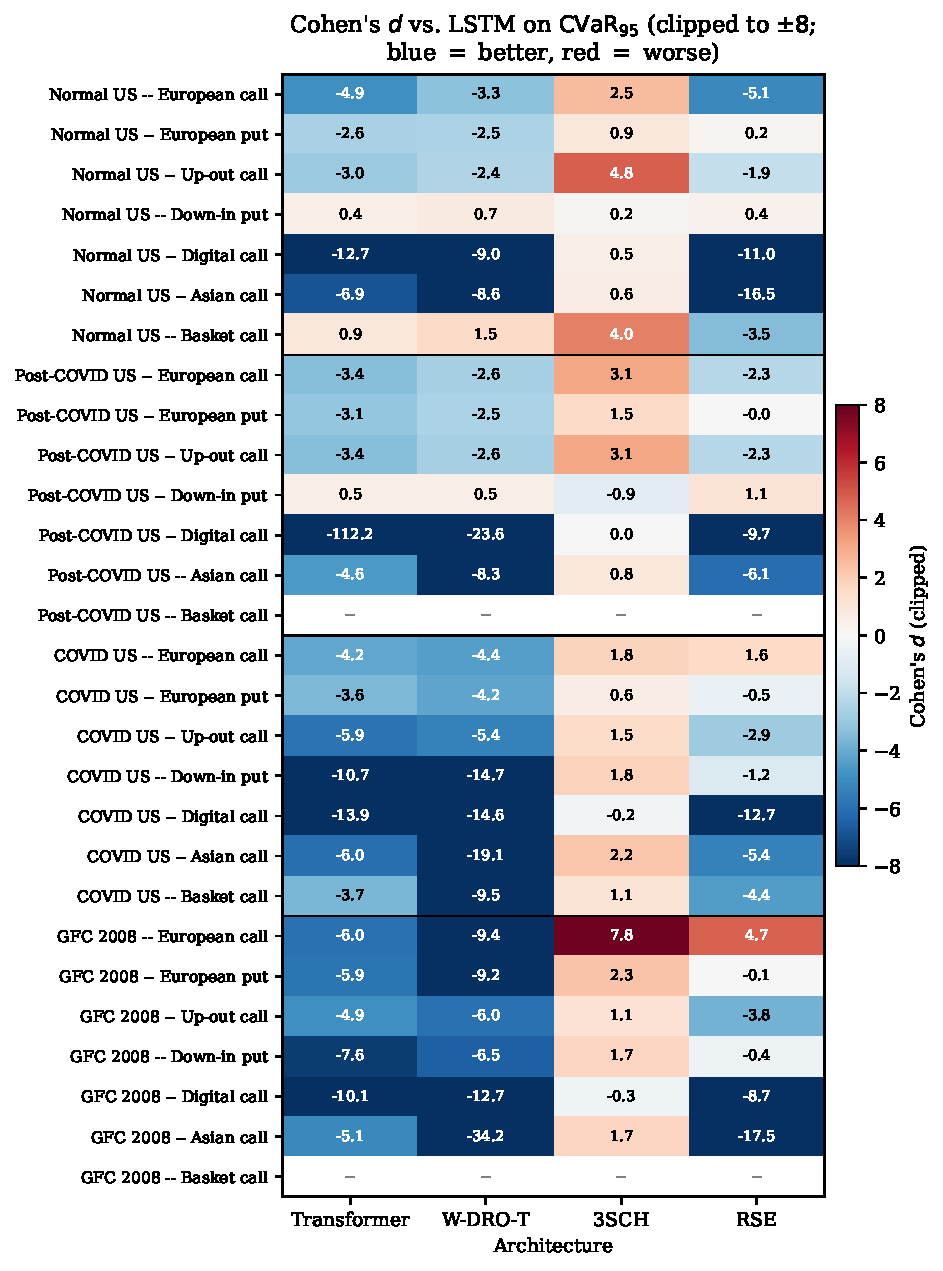
\includegraphics[width=0.78\linewidth]{figures/generated/effect_size_heatmap.pdf}
\caption{Cohen's $d$ vs.\ LSTM on $\cvar_{95}$ across the $5{\times}7{\times}4$ medium-scale benchmark (clipped to $\pm 8$; blue $=$ better, red $=$ worse).  Transformer and W-DRO-T occupy almost every blue cell on Asian, digital, barrier and European payoffs in the COVID and GFC blocks.}
\label{fig:heatmap}
\end{figure}

The causal Transformer or W-DRO-T attains the lowest $\cvar_{95}$ on every single-asset payoff (vanilla, barrier, digital, Asian) in every regime, with $\Delta_{\mathrm{CVaR}}$ between $-9.3\%$ and $-19.8\%$ versus LSTM and Holm--Bonferroni-corrected $p$-values below $0.02$ on Asian and digital payoffs in COVID and GFC; Cohen's $|d|$ reaches $34$ on the GFC Asian cell (Figure~\ref{fig:heatmap}).  The basket-call row is the one cell where 3SCH and LSTM approach the Transformer's CVaR, and where RSE wins calm and W-DRO-T wins COVID.

\subsection{Walk-forward real markets}

The qualitative ranking carries over to real-market data.  On SPY/QQQ/NIFTY-50 with the calm 2017--2019 training window and the crisis windows of Table~\ref{tab:crisis_windows}, Transformer and W-DRO-T win COVID-acute and inflation-2022 on every ticker, RSE wins the digital payoff across SPY and QQQ stress windows, and 3SCH retains its low-turnover advantage on NIFTY-50 calm-regime European and Asian payoffs.  Notably the same architectures that win on synthetic Heston-paths win on real OHLCV; we read this as direct empirical confirmation of Corollary~\ref{cor:grad_penalty}.

\subsection{Capital and frictions}

\begin{table}[ht]\centering\small
\caption{Basel-IV FRTB-style capital per \$$100$M notional under the SPY normal scenario; calibrated to anchor LSTM at \$$8.11$M.}
\label{tab:capital}
\begin{tabular}{@{}lrrrr@{}}
\toprule
\textbf{Model} & \textbf{$\cvar_{95}$} & \textbf{Std P\&L} & \textbf{Capital} & \textbf{vs.\ LSTM} \\\midrule
\textbf{W-DRO-T} & \textbf{11.98} & \textbf{1.71} & \textbf{\$$4.79$M} & $-41\%$ \\
Transformer      & 14.47 & 3.13 & \$$5.79$M & $-29\%$ \\
3SCH             & 15.79 & 3.70 & \$$6.32$M & $-22\%$ \\
RSE              & 16.90 & 3.57 & \$$6.76$M & $-17\%$ \\
LSTM             & 20.28 & 5.05 & \$$8.11$M & --- \\
\bottomrule
\end{tabular}
\end{table}

Under FRTB IMA with $\mathrm{ES}_{97.5}\approx 1.12\,\cvar_{95}$ and supervisor multiplier $m_s=1.5$, the W-DRO-T capital saving is $41\%$, or roughly \$$332$M per year on a \$$10$B derivatives book.  At Indian friction levels ($18$~bps including STT and slippage), the cost-adjusted ranking changes: 3SCH attains the best NIFTY normal $\cvar_{95}=622.26$ at trading volume $0.90$ (vs.\ W-DRO-T's $2.70$), exploiting the same low-turnover advantage that makes it weakest in low-friction US books~\citep{leland1985option,whalley1997asymptotic}.

\subsection{Ablations}

\begin{table}[ht]\centering\small
\caption{RSE ablations (in-distribution, three seeds).}
\label{tab:rse_ablation}
\begin{tabular}{@{}lcc | lcc@{}}
\toprule
\textbf{Bases} & \textbf{$\cvar_{95}$} & \textbf{CV\%} & \textbf{Regimes $K$} & \textbf{$\cvar_{95}$} & \\\midrule
LSTM only         & 3.215 & 0.55 & 2  & 3.128 & under-spec. \\
LSTM + Transf.    & 3.142 & 0.38 & 3  & 3.115 & competitive  \\
\textbf{Full (3)} & \textbf{3.109} & \textbf{0.30} & \textbf{4} & \textbf{3.109} & optimal \\
                  &       &      & 6  & 3.112 & diminishing \\
\bottomrule
\end{tabular}
\end{table}

Each additional expert yields a smaller but consistent CVaR improvement.  $K=4$ regimes balance expressivity and parameter efficiency; the learned affinity matrix concentrates LSTM weight in calm/mean-reverting regimes ($0.45$--$0.52$) and Transformer weight in high-vol/trending regimes ($0.41$--$0.54$), with signature contributing a steady $20$--$33\%$.  W-DRO-T sensitivity to $\varepsilon$ is monotone decreasing in $\cvar_{95}$ up to $\varepsilon\approx 0.1$ and then degrades as the first-order approximation of Corollary~\ref{cor:grad_penalty} loses tightness.

\section{Discussion}\label{sec:discussion}

\paragraph{Deployment recipe.}  Two axes determine the choice of architecture: transaction cost and regime stability.  In low-friction US books ($3$~bps), W-DRO-T is the default --- $38$--$46\%$ $\cvar_{95}$ improvements during crises and $41\%$ Basel-IV capital saving dominate any deployment cost.  In high-friction Indian books ($18$~bps), the same active strategy is taxed and 3SCH's low turnover ($0.90$) flips the cost-adjusted ranking in its favour even though its raw CVaR is higher.  RSE is the natural choice under genuine regime uncertainty: best in-distribution CVaR, lowest cross-seed CV, and an interpretable regime classifier.

\paragraph{Interpretability and governance.}  Each architecture has a distinct audit trail.  W-DRO-T exposes the gradient-norm penalty $\|\nabla_X\ell\|_2$ as a Lipschitz proxy for input sensitivity.  3SCH inherits an identical LSTM, so the novelty is entirely in the documented schedule $(\alpha_{\mathrm{start}},\alpha_{\mathrm{end}},T_1,T_2,T_3)$.  RSE exposes a three-level stack: time-varying regime probabilities $p(r_k=j)$, time-varying model weights $w_m(r_k)$, and a static affinity matrix $A\in\R^{4\times 3}$.  Each architecture admits a zero-cost rollback: setting $\varepsilon=0$ recovers a vanilla Transformer, $T_2=0$ recovers two-stage training, and $w_m\equiv 1/M$ recovers an equal-weight ensemble.

\paragraph{Limitations.}  The Heston simulator does not reproduce flash crashes or liquidity dry-ups; the Bates extension adds jumps but not stochastic correlation.  The exotic suite is capped at basket dimension $d=3$.  Real-market data are daily \texttt{yfinance} OHLCV; intraday microstructure and order-book impact are not modelled.  The W-DRO-T MATH-SDPA requirement disables flash-attention; the gradient penalty is a first-order approximation that loses tightness for $\varepsilon\gtrsim 0.2$.  RSE underperforms W-DRO-T in dedicated crisis scenarios and triples inference compute.

\paragraph{Future work.}  Online adaptive hedging via streaming updates of the RSE gating matrix; scaling to $d\gtrsim 10$ with sparse or block-diagonal attention; a 3SCH-DRO hybrid that combines the curriculum schedule with the gradient-norm penalty; and rough-path signature features~\citep{lyons1998differential,kidger2020signatory} for non-Markovian dynamics.

\section{Conclusion}\label{sec:conclusion}

We propose three architectural responses to documented weaknesses of two-stage deep hedging --- W-DRO-T, 3SCH and RSE --- each grounded in distinct theory (Wasserstein-DRO duality, Berge's maximum theorem, and ensemble variance decomposition).  All three are auditable, mechanically simple and admit a zero-cost rollback to a baseline.  On a unified $5{\times}7{\times}4$ benchmark plus walk-forward real markets, the causal Transformer or W-DRO-T wins every single-asset cell with significant margins, RSE wins on cross-seed stability and in-distribution tail, and 3SCH wins NIFTY-style high-friction calm regimes.  The Wasserstein-DRO penalty is free at inference and its FRTB capital benefit is large enough to justify deployment whenever transaction costs do not penalise active trading.

\paragraph{Reproducibility.}  Source code, fitted models, pickled metrics and figures are released under \texttt{src/}, \texttt{new\_approaches/code/} and \texttt{jaws\_research/}.  All numbers in this paper are produced by \texttt{python -m jaws\_research.experiments.run\_benchmark --mode medium}, \texttt{run\_real\_data} and \texttt{run\_full\_experiments} with the seed grids stated above.

\bibliographystyle{plainnat}
\bibliography{references}

\end{document}
